%\documentclass{beamer}
%\usetheme{Pittsburgh} 
\documentclass{scrartcl}

\usepackage[utf8]{inputenc}
\usepackage{default}
\usepackage[procnames]{listings}
\usepackage{graphicx}
%\usepackage[toc,page]{appendix}
\usepackage{caption}
\usepackage{hyperref}
\usepackage{color}

\usepackage{pdfpages}


%Bibliogrpahy?
\usepackage{bibentry}
%\nobibliography*
%\bibentry{ }


\begin{document}

\title{Assignment No. 8}
\subtitle{}
\author{
  Quignon, Christophe \\
  %Familyname, Name
} 
\date{\today}


\maketitle

\section{Read chapter 5.1 to 5.3 from Haykin’s book (2nd edition) and 5.4 till end from Haykin’s
book (3rd edition).
}

\begin{enumerate}
\item Radial-Basis Function Networks (RBFN)- Introduction

	\begin{itemize}
	\item In terms of NN, hidden units are a set of (RB)functions that for the basis for the input vectors.
	\item A RBNF consists of three layers:
		\begin{itemize}
		\item The input layer with the source nodes
		\item The hidden layer with the RBFs
		\item An Output layer 
		\end{itemize}

	\end{itemize}

\item Cover Theorem on the separability of patterns
	\begin{itemize}
	\item RBFNs solve classification tasks by non-linear transformation of the input to a higher dimensionality
	\item Covers theorem states that: A classification problem cast to a higher dimensionality is more likely to be linearly separable.
	\item The r-th order rationality varieties is defined as a mapping of by linearly r-wise products of the input
	\item Other separating surfaces are
		\begin{itemize}
		\item hyperplanes
		\item quadrices
		\item hyperspheres
		\end{itemize}
	\item Covers theorem has two mayor components:
		\begin{itemize}
		\item Nonlinear hidden functions
		\item High dimensionality of the hidden space
		\end{itemize}
	\item The XOR problem for example can be solved with the function $e^{-||x-t_{1}||^{2}}$
	\end{itemize}
	
\item Interpolation problem
	\begin{itemize}
	\item For RBNFs the choice of the nonlinear mapping is important
	\item For every learning process there are two major phases:
		\begin{itemize}
		\item Training phase, which optimizes the fitting procedure
		\item generalization phase, which finds an optimal fit between the two datasets
		\end{itemize}
	\item With multivariable interpolation, we gain the function to classify points.
	\item This can be done by all functions covered in Micchelli's theorem.
	\item Three functions are of interest to RBNFs:
		\begin{itemize}
		\item Multiquadrics Functions
		\item Inverse Multiquadrics Functions
		\item Gaussian Functions 
		\end{itemize}
	\item  Even though multiquadric functions grow at infinity can be used for a smooth input-output mapping
	\end{itemize}
	
\item RBFN
	\begin{itemize}
	\item An RBNF may be redundant if the input is directly mapped to hidden neurons, because their number is the same.
	\item RBFNs do not use back-propagation
	\end{itemize}
	
\item K-Means
	\begin{itemize}
	\item Clustering is a form of unsupervised learning
	\item This clustering is done by "encoding" (mapping)the input to smaller set of numbers
	\item K-Means clusters data to a set of nearest means.
	\item K-Means works iteratively with a given set of clusters and some guessed initial cluster centers.
	\item K-Means iterates two basic steps:
		\begin{itemize}
		\item Assign all point to their nearest cluster means.
		\item Move the cluster mean to the mean of all assigned points.
		\end{itemize}
	\item K-Means is locally optimal and thus often run with several initial guesses.
	\item in RBNFs K-Means is the nonlinear transformation of a hidden neuron
	\end{itemize}
	
\item Recursive least-mean-squares estimation of weight vectors
	\begin{itemize}
	\item Since K-Means runs recursively, we want to have a recursive version of LS estimation
	\item The algorithms is as follows:
		\begin{itemize}
		\item Calculate the prior estimation error
		\item Multiply by the weights to get the innovation
		\item Update weight vectors
		\end{itemize}
	\item This can also be reformulated in a recursive manner
	\end{itemize}
	
\item Hybrid learning procedure for RBFNs
	\begin{itemize}
	\item Combining K-Means and RLS we get a hybrid learning procedure
	\item This hybrid learning procedure consist of:
		\begin{itemize}
		\item Input layer with the size of the input dimensionality
		\item Hidden layer
			\begin{itemize}
			\item With the size of K from K-Means.
			\item With the cluster mean as the center for the Gaussian functions
			\item The same width $\sigma  = \frac{d_{max}}{\sqrt{2K}}$to all Gaussians
			\end{itemize} 
		\item Output layer by the RLS algorithm
		\end{itemize}
	\end{itemize}
	
\item Computer Experiment
	\begin{itemize}
	\item A classic example for computational experiments in pattern classification is the two-moons setting.
	\item comparing MLP and RBNFs performance on the two moons we conclude:
		\begin{itemize}
		\item RBFN outperforms MLP
		\item RBFN are computationally faster than MLP
		\end{itemize}
	\end{itemize}
	
\item Interpretations of the Gaussian hidden units
	\begin{itemize}
	\item In neurobiology sensors have receptive field where they fire with a certain probability.
	\item Those receptive field follow a Gaussian model and correspond to Gaussian hidden units in NNs
	\item Gaussians can also be interpreted as Kernels, since they share the same properties:
		\begin{itemize}
		\item It is continuously bounded real function symmetric to the origin, where the max value is.
		\item The total order under the surface is one
		\end{itemize}
	\end{itemize}
	
\item Kernel regression and its relation to RBFNs
	\begin{itemize}
	\item Instead of interpolation we can user density estimation or kernel regression
	\item This estimator has to be asymptotically unbiased
	\item The Parzen-Rosenblatt density estimator does exactly this.
	\item The regression function can be estimated by:
		\begin{itemize}
		\item Nadaraya-Watson regression estimator
		\item Normalized RBFNs
		\end{itemize}
	\end{itemize}
	
\item Summary and discussion
	\begin{itemize}
	\item The main difference between RBFN and MLP is that MLPs use weighted summmations and RBFNs use a single weighted sum.
	\item K-Means RLS and SVM have a nearly identical performance.
	\item For both nonlinear regression models, the Nadaraya-Watson and the normalized RBF, multivariate Gaussians are a good choice for the kernel.
	\end{itemize}
\end{enumerate}



\section{Without the use of Cover theorem, determine the probability P(N, m1) that a binary partition(C1, C2) of training set picked at random is linearly separable in a feature space of dimension m1 for the following two cases:
}
\subsection{ m1 = 1, N = 3
}
Possible cases:\\
ooo = separable\\
oox = separable\\
oxo = non-separable\\
oxx = separable\\
xoo = separable\\
xox = non-separable\\
xxo = separable\\
xxx = separable\\
$\to 6/8$ or $0.75\%$ of the cases are separable.


\subsection{ m1 = 2, N = 3
}
In 2-D, there is no give a probability to the alignment of randomly chosen point being in a line. In that case the upper probability would hold\\
But it is very unlikely that all point fall on a line, and thus the over all probability of non-separability is very low.

\subsection{Check the result you obtain is equal to the one derived by using formula of Cover
theorem.
}

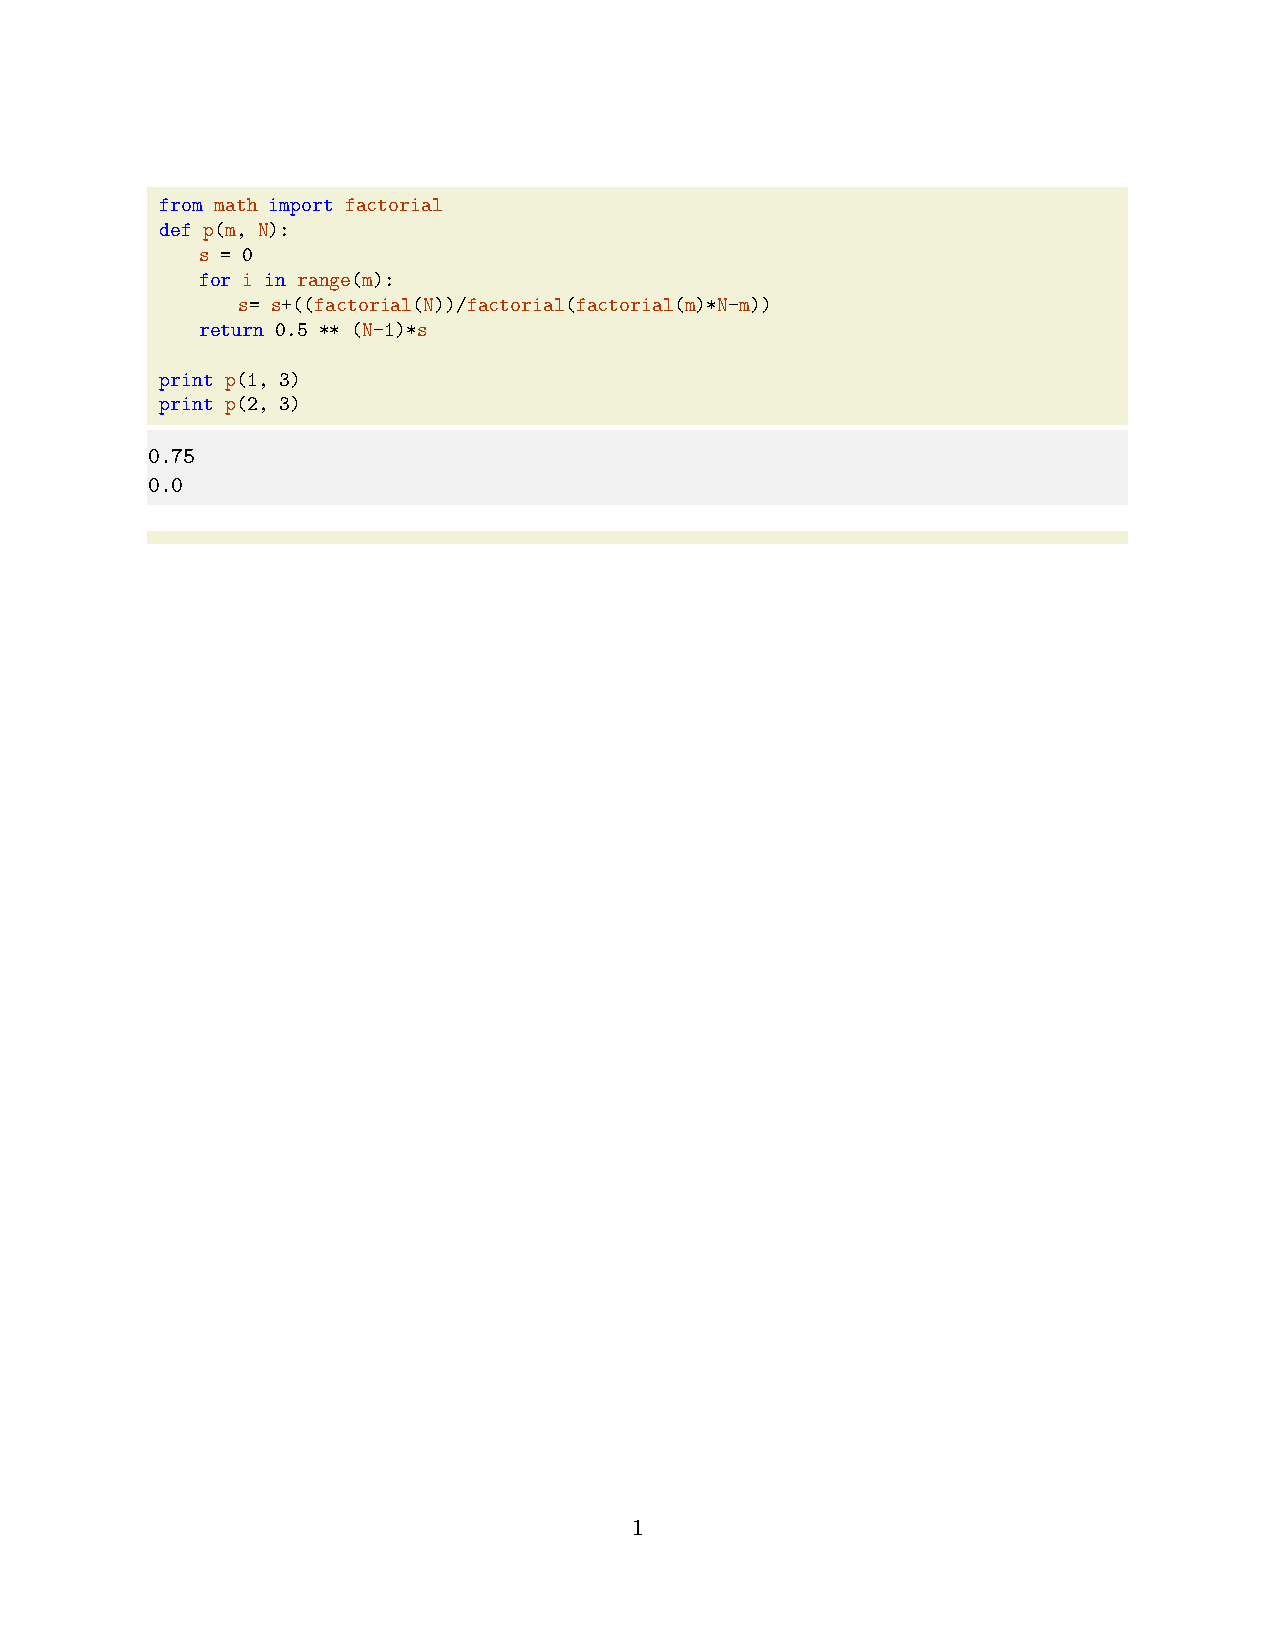
\includepdf[pages={1-},scale=1]{cT.pdf}

\section{}
\subsection{ Consider the two classes C1 = \{-1, 1\}, C2 = \{0\}}
\subsubsection{Are C1 and C2 linearly separable?}
No
\subsubsection{ Use a RBF neural network to construct a feature space where C1 and C2
become linearly separable.}
With $y(x) = x^{2}$

\subsection{Consider now the two classes C1 = \{-1, 1\}, C2 = \{-2, 0\}}
\subsubsection{Are C1 and C2 linearly separable?}
No
\subsubsection{Use a RBF neural network to construct a feature space where C1 and C2
become linearly separable.}

With $y(x) = 2x^{3} +3x^{2} - 1x$

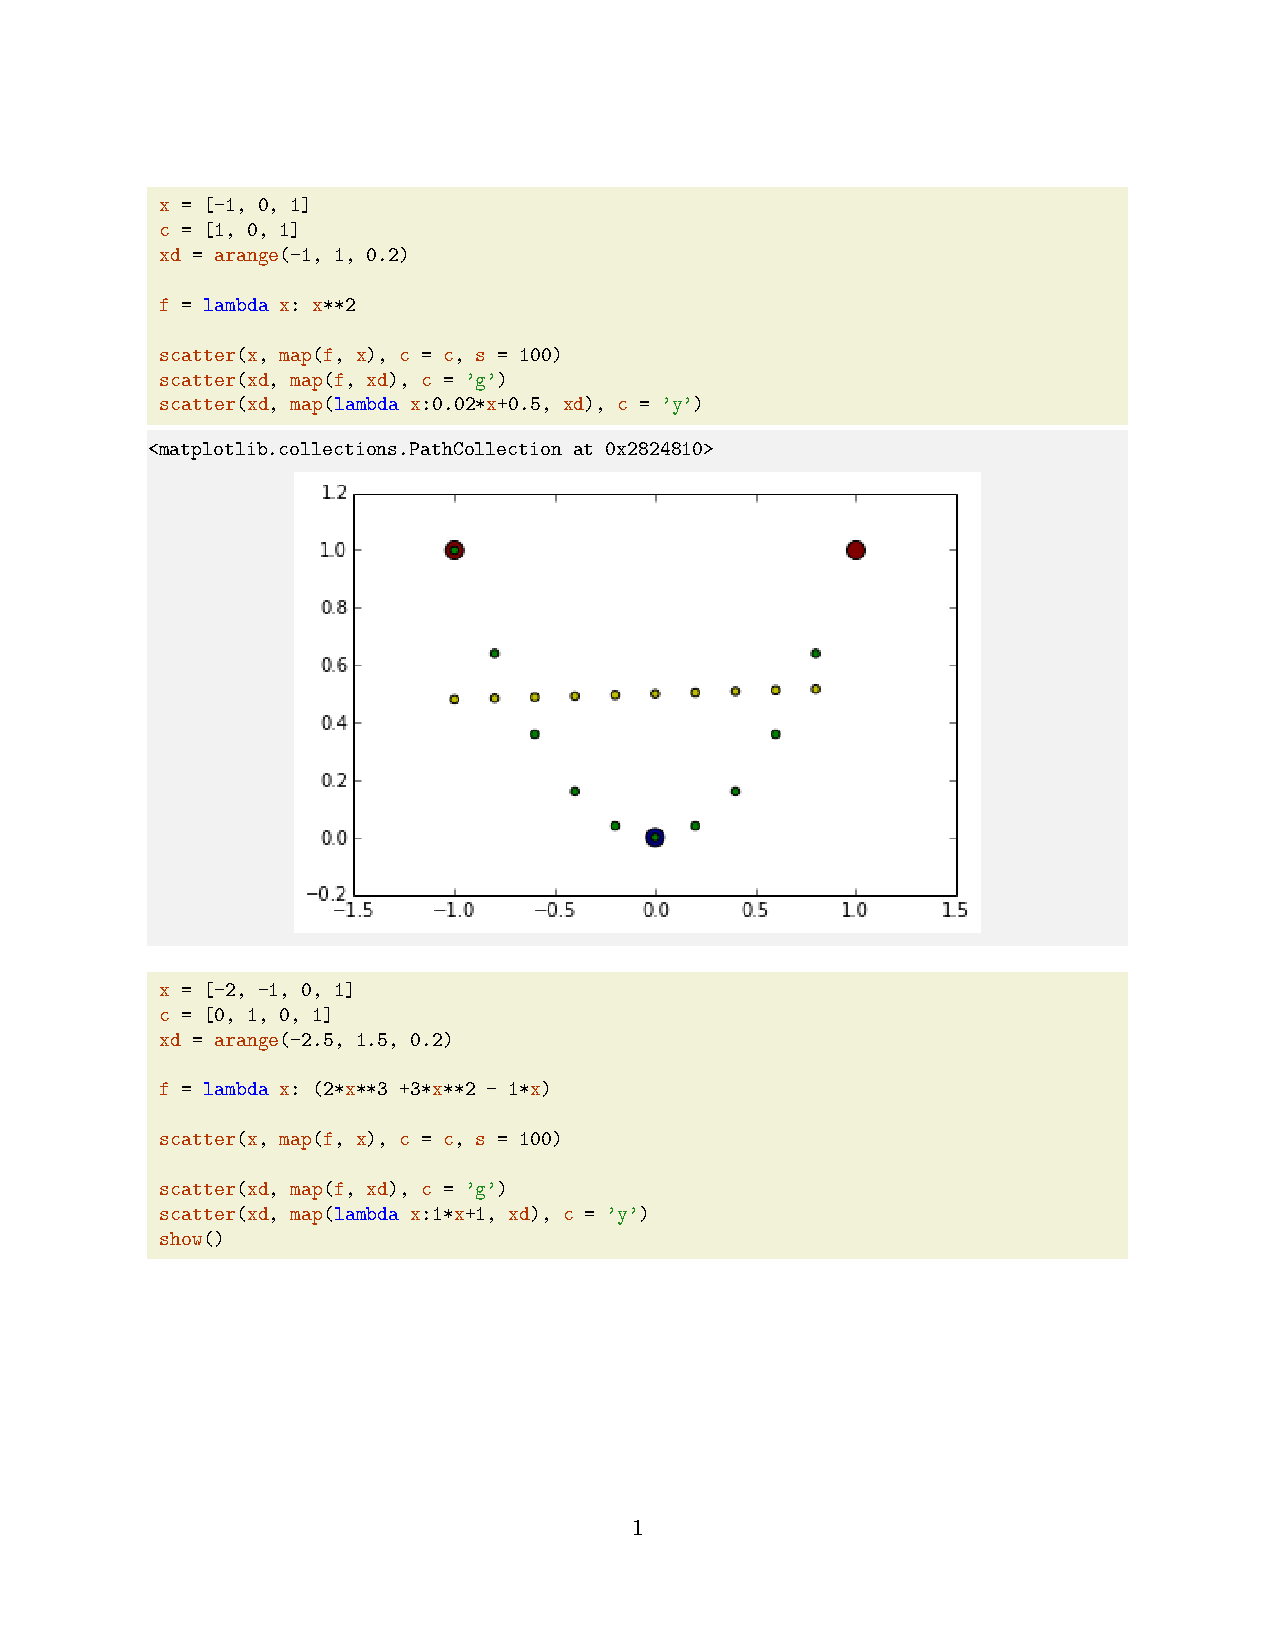
\includepdf[pages={1-},scale=1]{separate.pdf}


\section{}
\subsection{ In this experiment you have to implement a radial basis function network.}

\subsection{Test case of your network: Now do the "Double moon" experiment described in the
previous assignment using your RBF network.}

 Experimenting on only two cases are
enough.
\begin{itemize}
\item When the moons are close enough but not touching.
\item Each moon partially overlaps each other.
\end{itemize}
Vary the number of centers, regularization parameter lambda and present your results
with comments:\\

Lambda 0.2 is agood choice for the first run.\\
For K $\geq$ 7, K-Means fails.\\
For non-overlapping moons, K = 3 is fine.\\
For overlapping moons, K=5 performs fine.\\

In conclusion, K and lambda are problem specific and have to fine tuned at the same time.

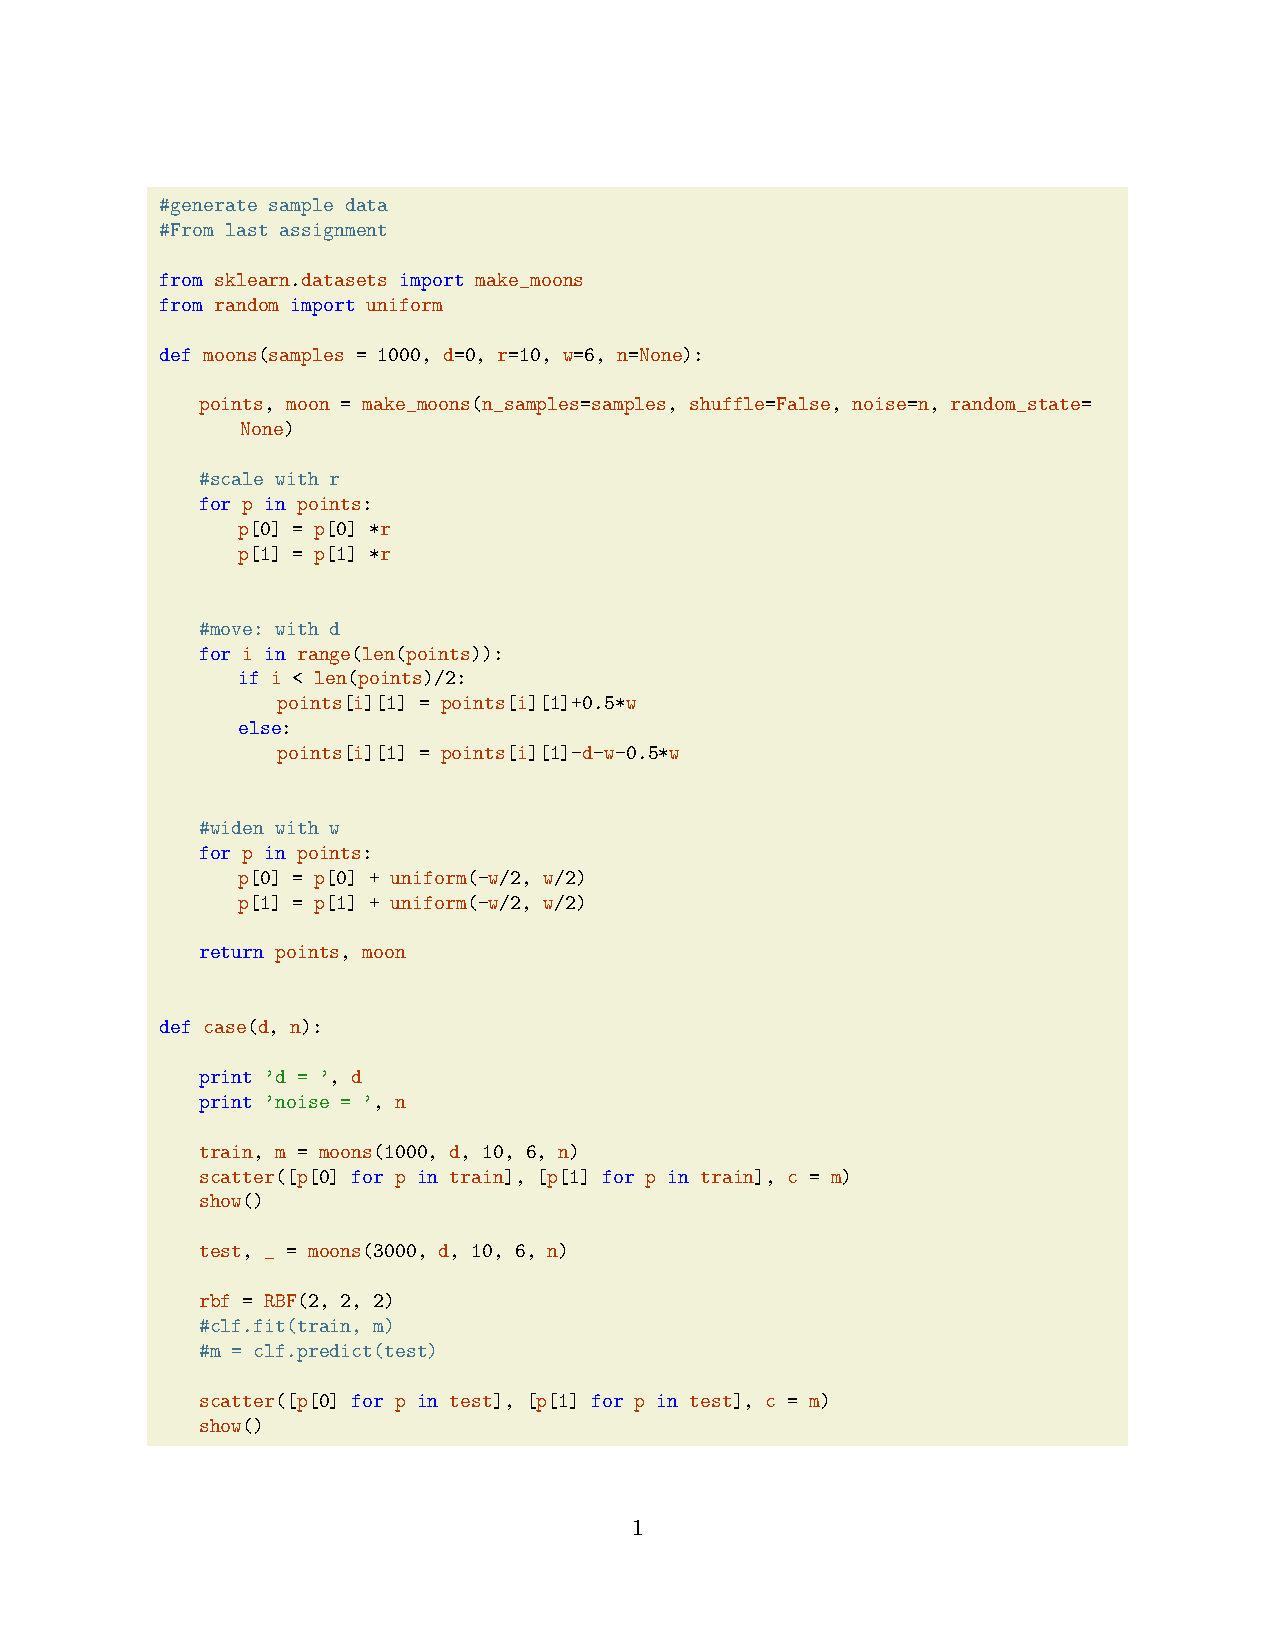
\includepdf[pages={1-},scale=1]{Ex8.pdf}


%CONTENTS
%NOTES


%COPY AND PASTE FROM HERE

%\begin{enumerate}
% \item 
%\end{enumerate}

%\hyperref{link}{text}

%\begin[Language=Python]{lstlisting}
%#PYTHON CODE HERE
%\end{lstlisting}

%\lstinputlisting[Language=Python]{ }

%\begin{figure}
% \center
% \includegraphics[width= cm]{ }
% \caption{}
%\end{figure}

%BIBLIOGRPAHY?
\bibliographystyle{plain}%amsalpha
\bibliography{Top30.bib}
%\bibentry{}

\end{document}
